    %Document type
\documentclass[12pt, a4paper]{report} %options include: article (use for small reports and essays, report (use for thesis), book (maybe better for thesis?), slides (lul wut)
\usepackage{caption}
\usepackage{subcaption}
\usepackage[a4paper,width=150mm,top=25mm,bottom=25mm, bindingoffset=6mm]{geometry}
\usepackage{titlesec}    
\titleformat{\chapter}[display]
{\normalfont%
    \huge% %change this size to your needs for the first line
    \bfseries}{\chaptertitlename\ \thechapter}{10pt}{%
    \Large %change this size to your needs for the second line
    }
\usepackage{lipsum}%Just for testing structure, isn't needed for final work
    %header/footer
\usepackage{fancyhdr}%headers and footers package
%\pagestyle{fancy}
\pagestyle{plain}
\lhead{MRes Biology}%left header
%\chead{}%centre header
\rhead{Bloggs, J. 2016}%right header
%\lfoot{}%left footer, etc etc
%\cfoot{}
%\rfoot{}
\renewcommand{\headrulewidth}{0.4pt}%line thickness for header
\renewcommand{\footrulewidth}{0.0pt}%as above, for footer

\usepackage[utf8]{inputenc}%language package, must be on
\usepackage{amsmath}%maths package, keep on for greek letters, numbers stuff.
\usepackage{textcomp} %For typing the degrees symbol. "\textdegree C"
\usepackage[]{natbib}%referencing package (DO NOT FUCK THIS)
\usepackage{setspace}%linespacing
\doublespacing  %1.5 line spacing is a safe bet, I'd stick with it 
\usepackage{graphicx}%allows images to be inserted
\graphicspath{ {images/} }%directory where image files are kept for the compiler
\usepackage{seqsplit}%For Fasta sequences or something like that- use \seqsplit{sequencehere}
%\usepackage[none]{hyphenat}%Prevents words being split across lines. Optional
    
\usepackage{hyperref}%Makes contents page lines and citations in text clickable links
\hypersetup{
    colorlinks=true,
    citecolor=blue,%citation colour
    filecolor=black,
    linkcolor=black,%contents page colour
    urlcolor=black
}

\usepackage{afterpage}
    %Document particulars
\title{Insert title here}
\author{Ryan Buttery}
\date{Insert date here}

\fancypagestyle{plain}{%
    \lhead{MRes Biology}
    \rhead{Buttery, R.D. 2016}
    \fancyfoot[C]{\thepage}%
\renewcommand{\headrulewidth}{0.4pt}% Line at the header invisible
\renewcommand{\footrulewidth}{0.0pt}% Line at the footer visible
}
\begin{document}
    %Don't mess with these!
\bibliographystyle{apa} %seems to be the closest to what I normally do. Need to experiment with books still though. Probably fine!
\setcitestyle{round} %makes the brackets on citations round like (this)
\renewcommand{\bibname}{References}

%Which levels of section are shown in contents (0=chapter, 1=section, 2=subsection, etc)
\setcounter{tocdepth}{3}
%Which levels should be numbered. Chapter 1, section 1.1, etc
\setcounter{secnumdepth}{0}
\renewcommand{\familydefault}{\rmdefault}


%%%UNCOMMENT THE FOLLOWING LINES AS THEY ARE COMPLETED AND/OR REQUIRED

\pagenumbering{gobble}%Hides page number on verso (back) of cover page
\begin{titlepage}
    \begin{center}
        \vspace*{1cm}
        
        \Large
        \textbf{PROJECT TITLE IN BIG LETTERS COR BLIMEY LOOK AT THIS SCIENCE}
        
        \vspace{0.5cm}
        \large
       A subtitle, you know.. if you're into that kind of thing
        
        \vspace{1.5cm}
        
        \textbf{Joe Bloggs}
        
        \vfill
        
        A thesis presented as part requirement for the\\
        degree of Master of Research in Biology
        
        \vspace{0.8cm}
        
        
\includegraphics[width=0.4\textwidth]{university}
        
        \Large
        Institute of Science and the Environment\\
        University of Worcester\\
        United Kingdom\\
        2016
        
    \end{center}
\end{titlepage}
\newgeometry{a4paper,width=150mm,top=25mm,bottom=25mm,bindingoffset=-6mm, twoside}%This is setup for binding already, comment out if making a PDF version for electronic submission
\afterpage{\null\newpage}

\chapter*{Abstract}
\pagenumbering{roman}%Makes prefaces have roman numerals
A Few notes for you. This has automatically generated tables of contents, figures, and tables. This uses Bibtex referencing, so have a little look at that. (Download mendeley omg). It is ready for binding as far as I'm aware, the binding offset is already in place, so print away. (Perhaps do the first 5 pages first on duplex, just to double check though!!). Good luck, and may the force be with you.
\addcontentsline{toc}{chapter}{Abstract}%adds un-numbered chapter to contents page
\setcounter{page}{1}%Tells it to start counting numbers from here


\addcontentsline{toc}{chapter}{Prefaces}

\chapter*{Dedication}
\addcontentsline{toc}{section}{Dedication}
I dedicate this work to my parents etc etc...


\chapter*{Acknowledgements}
\addcontentsline{toc}{section}{Acknowledgements}
I wish to acknowledge and express my sincere gratitude to the following individuals for their invaluable assistance in the completion of my project:
\begin{itemize}
    \item Batman
    \item James Bond
    \item Deckard off of Bladerunner
    \item Éowyn for taking care of the Nazgûl's leader
\end{itemize}

\newpage
\addcontentsline{toc}{section}{Table of Contents}
\tableofcontents

\listoffigures
\addcontentsline{toc}{section}{Figures}

\listoftables
\addcontentsline{toc}{section}{Tables}

\chapter*{Table of Abbreviations}
\input{prefaces/abbreviations}
\pagestyle{fancy}


\chapter{Introduction}
\pagenumbering{arabic}%Makes page numbers normal
\section{Introduce Concepts and Ideas required to understand project in context}
\lipsum %delete this, just makes placeholder text.
\section{My Project}
\lipsum %delete this, just makes placeholder text.
\section{Aims and Objectives}
\begin{enumerate}
    \item Obj 1
    \item Obj 2
    \item Etc etc..
\end{enumerate}

\chapter{Title}%Chapter 2 title here
\section{Introduction}
\lipsum %delete this, just makes placeholder text.
Let's cite something in brackets \citep{Kearse2012geneious}. Let's cite two in brackets \citep{Kearse2012geneious, Belhaj2013}.

Let's add a figure of what the lac operon does because I have it to hand. See Figure \ref{fig:lacbanter}.
\begin{figure}[h]
    \centering
    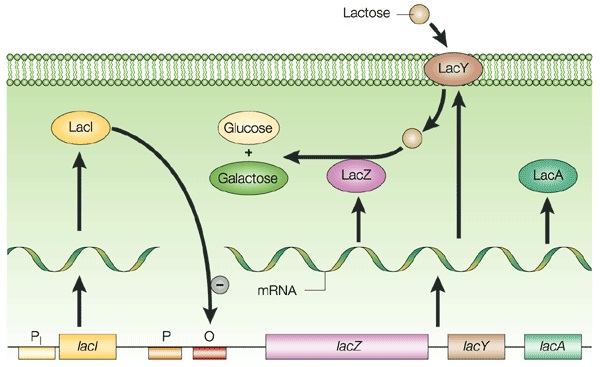
\includegraphics[width=0.6\textwidth]{lac.jpg}%width=1.0 is textwidth.
    \caption{Example figure.}
    \label{fig:lacbanter}%this is a unique identifier for this figure. Allows you to reference it in the text.
\end{figure}

Now let's insert a table, ya know, because we can. See Table \ref{tab:spam}.

\begin{table}[h]
\centering
\caption{Example table}
\label{tab:spam}
\begin{tabular}{|l|l|}
\hline
A thing & Another thing \\ \hline
Eggs    & 0             \\ \hline
SPAM    & 100+          \\ \hline
\end{tabular}
\end{table}
\section{Methods}
\lipsum %delete this, just makes placeholder text.
\newpage
\section{Results}
\lipsum %delete this, just makes placeholder text.
\newpage
\section{Discussion}
\lipsum %delete this, just makes placeholder text.
\newpage
\section{Main findings}
\lipsum %delete this, just makes placeholder text.

\chapter{Title}%Chapter 3 title here
\section{Introduction}
Let's cite something in brackets \citep{Kearse2012geneious}. Let's cite two in brackets \citep{Kearse2012geneious, Belhaj2013}. According to \citet{weber2011modular}, I can cite in text this way.. (Use , to add a second.. or more if you're into that kind of thing)
\section{Methods}
\lipsum %delete this, just makes placeholder text.
\newpage
\section{Results}
\lipsum %delete this, just makes placeholder text.
\newpage
\section{Discussion}
\lipsum %delete this, just makes placeholder text.
\newpage
\section{Main findings}
\lipsum %delete this, just makes placeholder text.

\chapter{Discussion of findings}
\lipsum
\lipsum


\chapter{Conclusions}
\begin{itemize}
    \item Conclusion 1
    \item 2
    \item buckle my shoe
    \item you know the drill
\end{itemize}


%%%BIBTEX REFERENCING%%%
\pagestyle{plain}
\newpage
\addcontentsline{toc}{chapter}{References}
\bibliography{references.bib} %make sure to keep references in a file called "references.bib"


\newpage
\appendix
\chapter{Name of first Appendix}
\subsection{Subsection 1}
\subsubsection{Sub-Subsection inception}
\begin{verbatim}
>Example_Fasta_Sequence
\end{verbatim}
\seqsplit{GTTTTAGAGCTAGAAATAGCAAGTTAAAATAAGGCTAGTCCGTTATCAACTTGAAAAAGTGGCACCGAGTCGGTGCTTTTTTTCTAGACCCAGCTTTCTTGTACAAAGTTGGCATTA}
\subsubsection{another one}
\begin{verbatim}
>Fasta_2
\end{verbatim}
\seqsplit{GCTAACAACATAAAACTTGTTGGGTTTTAGAGCTAGAAATAGCAAGTTAAAATAAGGCTAGTCCGTTATCAACTTGAAAAAGTGGCACCGAGTCGGTGCTTTTTTTCTAGACCCAGCTTTCTTGTACAAAGTTGGCATTA}
\chapter{Another appendix. You get the idea}



\end{document}
%useful instructions

%CITING AND REFERENCING
%to cite: \citep{} for bracketed, \citet{} for no brackets, \citep{1,2,...) for multiple
%Don't forget to give your references in references.bib a suitable codename before trying to cite them like a spanner!
%See http://ctan.org/pkg/natbib for citation help!

%MISC
%Detexify is a beautiful thing for symbols! http://detexify.kirelabs.org/classify.html
%When using greek letters, like in microliters, do it like this: 1.5$\mu$l
%MAKE TABLES WITH THIS http://www.tablesgenerator.com/